
\chapter{The Land Surface Climate in the Regional Arctic System Model}
\label{chap:land_surface}

This chapter has been published in its current form in the \textit{Journal of Climate}.
\textcopyright American Meteorological Society.
Used with permission.
\begin{itemize}
    \item \bibentry{Hamman_2016a}.
\end{itemize}

The supplemental material for this chapter is provided in appendix \ref{chap:land_surface_sup}.

{\bf Abstract}
The Regional Arctic System Model (RASM) is a fully coupled, regional Earth system model applied over the pan-Arctic domain.
This paper discusses the implementation of the Variable Infiltration Capacity land surface model (VIC) in RASM and evaluates the ability of RASM, version 1.0, to capture key features of the land surface climate and hydrologic cycle for the period 1979–2014 in comparison with uncoupled VIC simulations, reanalysis datasets, satellite measurements, and in situ observations.
RASM reproduces the dominant features of the land surface climatology in the Arctic, such as the amount and regional distribution of precipitation, the partitioning of precipitation between runoff and evapotranspiration, the effects of snow on the water and energy balance, and the differences in turbulent fluxes between the tundra and taiga biomes.
Surface air temperature biases in RASM, compared to reanalysis datasets ERA-Interim and MERRA, are generally less than 2$^{\circ}$C; however, in the cold seasons there are local biases that exceed 6$^{\circ}$C.
Compared to satellite observations, RASM captures the annual cycle of snow-covered area well, although melt progresses about two weeks faster than observations in the late spring at high latitudes.
With respect to derived fluxes, such as latent heat or runoff, RASM is shown to have similar performance statistics as ERA-Interim while differing substantially from MERRA, which consistently overestimates the evaporative flux across the Arctic region.

\section{Introduction}
\label{sec:intro_ch3}

The Regional Arctic System Model (RASM) is a fully coupled regional Earth system model \citep{Roberts_2015a} applied over the pan-Arctic domain (Fig. \ref{fig:domain}a).
The development of RASM has been motivated by the need to improve the representation of critical Arctic processes and feedbacks that affect multidecadal simulations of high-latitude climate, to advance understanding of the coupled interactions between components within the Arctic climate system, and ultimately to better understand climate change at high latitudes.
In RASM, the land surface scheme is the Variable Infiltration Capacity model \citep[VIC; ][]{Liang_1994,Liang_1996}, which is coupled to atmosphere, ocean and sea ice model components via the Community Earth System Model \citep[CESM;][]{Hurrell_2013} flux coupler software infrastructure \citep{Craig_2012}.

\begin{figure}
  \centering
  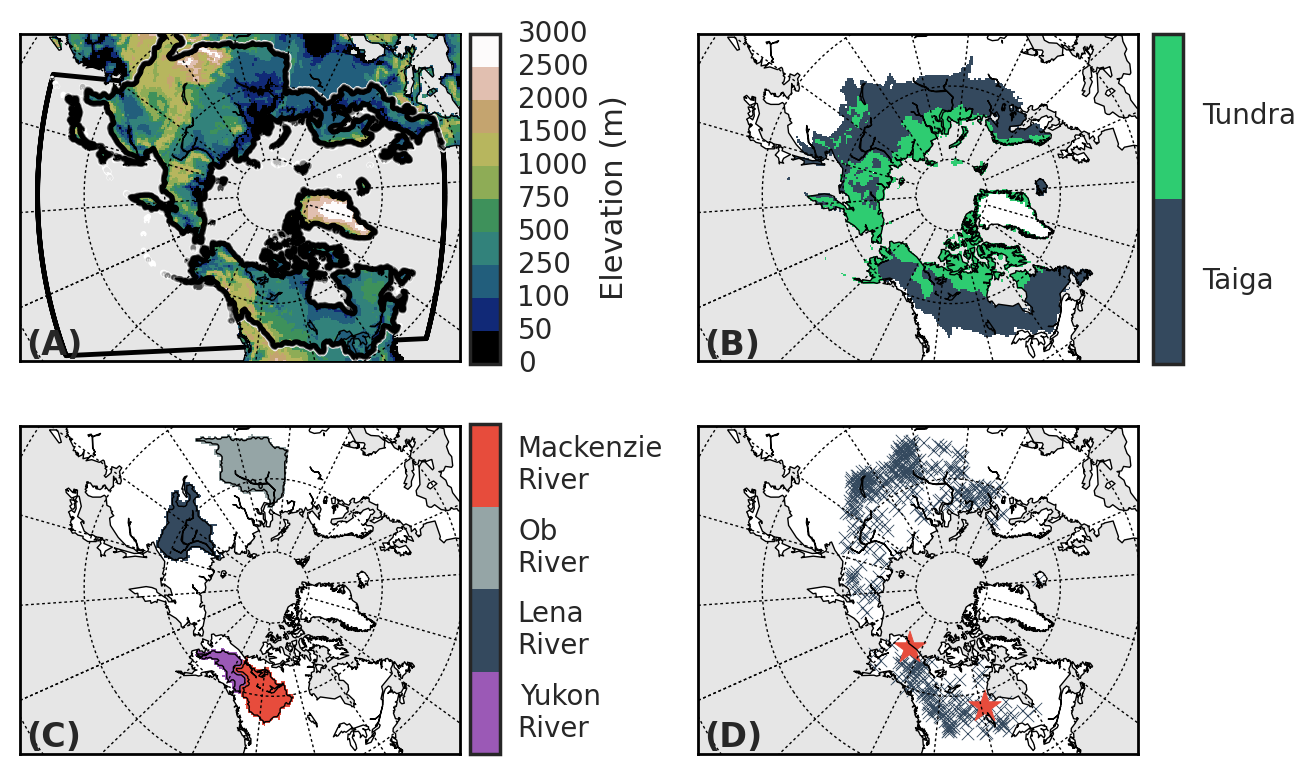
\includegraphics[width=12cm,keepaspectratio]{ch3_Fig1}
  \caption{(a) Domain of the Regional Arctic System Model.
  The 50-km near-equal-area land and atmosphere domain is shown as the outer boundary.
  Shaded areas represent the topographic height for individual land model grid cells.
  The black contour defines the RVIC drainage area over land, and the 1/12$^{\circ}$ inner ocean-ice domain over the ocean.
  (b) The tundra and taiga biomes in the RASM domain.
  (c) The Mackenzie, Ob, Lena, and Yukon River basins.
  (d) The location of R-ArcticNET streamflow gauges (dark blue crosses) and AmeriFlux towers (red stars) used in this analysis.}
  \label{fig:domain}
\end{figure}

We assess the RASM-simulated land surface climate and land–atmosphere coupling in terms of a range of hydrometeorological variables.
We compare fully coupled simulations using RASM version 1.0 to reanalysis, remote sensing, and observation-based datasets.
Our goal in this paper is to establish a baseline for future model development and applications, and to understand the processes that are and are not well represented.

The Arctic land surface plays three primary roles in the global climate system.
First, most of the Arctic land surface has a negative net radiation flux and thus acts as a heat sink, balancing the poleward heat flux from lower latitudes \citep{Fasullo_2008}.
Second, the high albedo in the Arctic during periods of snow cover controls the net shortwave flux in the regional surface energy balance \citep{Flanner_2011}.
Declines in the regional albedo associated with reductions in snow and ice cover therefore contribute to the process of polar amplification \citep{Serreze_2006c}.
Finally, by most accounts, the runoff from the Arctic land surface provides the largest freshwater flux into the Arctic Ocean \citep{Serreze_2006a}.
This flux lowers the salinity in the Arctic Ocean, which is important for sea ice development and is a driver of coastal, regional, and global ocean currents originating in the Arctic Ocean \citep{Morison_2012,Serreze_2006a}.

The land surface hydroclimate in the pan-Arctic region has been extensively studied using offline (uncoupled) hydrologic model simulations.
For example, \citet{Slater_2007} forced five uncoupled land surface models with the ECMWF reanalysis called ERA-40 over the pan-Arctic drainage area.
They cited intermodel differences of up to 30\% in the partitioning of precipitation into evapotranspiration and runoff.
They also noted that most models struggled to capture the winter baseflow behavior, deficiencies that were partially corrected, in some of the models, by adjusting the soil parameterizations.
\citet{Adam_2007} and \citet{Tan_2011} used uncoupled implementations of VIC to investigate twentieth-century changes in annual and seasonal hydrologic fluxes in the Arctic.
Frequently, uncoupled simulations are used to develop new model physics and to improve land surface process representations \citep{Bonan_2011,Bowling_2004,Bowling_2010,Cherkauer_2003,Swenson_2012}.
These studies have been useful in evaluating the model representations of hydrologic processes such as streamflow or evapotranspiration, but have not accounted for coupled land–atmosphere feedbacks.

The development of coupled land–atmosphere and Earth system models has been an important advance in our understanding of hydrometeorology.
Regional and global coupled land–atmosphere models offer a tool to understand how feedbacks between model components propagate changes in individual elements.
Notable examples of this can be found in numerous studies at high and middle latitudes that have shown the importance of antecedent soil moisture and surface albedo in seasonal climate forecasts \citep{Beljaars_1996,Betts_2004,Dominguez_2006,Koster_2004}.
Studies such as these highlight the importance of developing and evaluating land surface processes within a coupled model framework.

In this paper we describe the land surface component coupled within RASM, and evaluate the baseline behavior and performance of the RASM land surface scheme.
Section \ref{sec:models_ch3} provides a brief overview of RASM and the land surface model VIC.
Section \ref{sec:data_ch3} describes the model simulations and comparison data used in this analysis.
Section \ref{sec:results_ch3} presents the results from our analysis, comparing RASM simulated spatial fields to reanalysis and observation-based data products.
Section \ref{sec:discussion_ch3} presents a discussion of our results, using streamflow observations to constrain the partitioning of the hydrologic fluxes.
Section \ref{sec:discussion_ch3} also compares RASM surface fluxes directly to surface observations at selected flux towers, assessing the model’s ability to simulate the observed surface energy balance and diurnal cycle.
Finally, section \ref{sec:conclusions_ch3} states our conclusions and outlines the future applications and development intended for the RASM model.

\section{Model description}
\label{sec:models_ch3}

\subsection{RASM}

RASM is a high-resolution, regional, coupled Earth system model that has been developed to improve the representation of critical Arctic process and feedbacks that affect multidecadal simulations of climate in the pan-Arctic domain.
RASM version 1.0 uses the Community Earth System Model (CESM) coupling infrastructure \citep[CPL7; ][]{Craig_2012,Roberts_2015a} and is composed of five component models:

\begin{enumerate}
  \item The Weather Research and Forecasting (WRF) Model \citep{Skamarock_2008} is an atmospheric mesoscale meteorological model. \citet{DuVivier_2016} and \citet{Cassano_2016} provide a detailed description of the WRF model, version 3.2, as it is applied in RASM. Temperature and winds in the top 20 levels of WRF are spectrally nudged to scales larger than approximately 3400 km with nudging linearly ramped from no nudging at level 20 to a nudging strength of 0.0003 s−1 (nudged toward boundary conditions every 55 min) at level 40 \citep{Glisan_2013,Skamarock_2008}.
  \item The Parallel Ocean Program model \citep[POP; ][]{Smith_2010} is a general circulation ocean model. \citet{Roberts_2015a} provide a description of the application of POP, version 2, within RASM.
  \item The Los Alamos Sea Ice model \citep[CICE; ]{Hunke2015} is widely used in regional and global climate simulations. \citet{Roberts_2015a} provide a description of the application of CICE, version 5, within RASM.
  \item The streamflow routing model used is an adapted version of a linear routing model frequently used to route streamflows from VIC output \citep[RVIC; ][]{Lohmann_1996,Lohmann_1998b}. \citet{Hamman_2016b} provide a description of RVIC, version 1.0, as it is applied in RASM.
  \item The Variable Infiltration Capacity model \citep[VIC; ][]{Liang_1994,Liang_1996} is a macroscale hydrologic model. A more detailed description of VIC is provided in section \ref{sec:vic}.
\end{enumerate}

In RASM version 1.0, the land, atmosphere, and runoff components are configured on a 50-km near-equal-area North Pole stereographic grid.
The ocean and sea ice models are configured on a 1/12$^{\circ}$ rotated stereographic grid.
Each model exchanges fluxes with the coupler every 20 minutes \citep{Roberts_2015a}.

\subsection{VIC}
\label{sec:vic}

VIC is a semidistributed hydrologic model that solves the water and energy balance equations at the land surface.
VIC represents subgrid variability in vegetation and topography through a mosaic-style statistical tiling scheme.
Infiltration capacity is nonlinearly distributed \citep{Zhao_1980} and flow from the upper layer is driven by gravity to the lower layers according to \citep{Campbell_1974}.
Base flow is generated from the bottom soil layer and recedes nonlinearly as a function of soil moisture \citep{Dumenil_1992,Todini_1996}.
VIC does not consider direct interactions between neighboring cells, instead assuming that surface and subsurface runoff reach the channel before leaving the grid cell.
In RASM, runoff fields are passed to the flux coupler and are then routed to the Arctic Ocean using RVIC.

When run in energy balance mode, as it is in RASM, VIC uses an iterative process to determine the land surface temperature that minimizes the surface energy balance error \citep{Liang_1999}.
Accumulation and ablation of the snowpack are modeled using a quasi-two-layer snow model, consisting of a thin surface layer and a thicker pack layer \citep{Andreadis_2009,Cherkauer_1999}.
The full energy balance is computed for the surface layer, which exchanges fluxes with the atmosphere, while the pack layer is treated as a reservoir for mass and energy (cold content).
Change in snow water equivalent is the net result of snow, rain, throughfall, sublimation (or condensation), and melt.
Intercepted snow accumulates as a function of the leaf area index and canopy temperature \citep{Storck_2002}.
Snow albedo decays as a function of time and season \citep{Andreadis_2009}.

As an uncoupled hydrologic model, VIC has been applied at global and continental scales \citep{Maurer_2001,Nijssen_1997,Nijssen_2001} including numerous pan-Arctic hydrologic studies \citep{Adam_2007,Slater_2007,Su_2005,Tan_2011}.
VIC has also been coupled to prognostic atmospheric models, such MM5 \citep{Zhu_2009}, to provide lower boundary conditions over land.

RASM uses a modified implementation of VIC, version 4.0.4 (available at https://github.com/UW-Hydro/VIC/releases/tag/VIC.4.0.4).
Extensive structural changes to the VIC source code were required to allow coupling with other RASM component models via the flux coupler, but changes to the physical core of the model were limited.
The VIC physics used within RASM differs from the standard release version 4.0.4 in the following four major ways:

\begin{enumerate}
  \item Vegetation-dependent broadband albedo for snow: VIC typically treats snow-covered vegetation as a completely covered snow surface with a broadband albedo for new snow of 0.85. In early RASM simulations, this led to significant positive biases in surface albedo and consequent negative biases in net shortwave radiation and surface air temperature, especially in coniferous vegetation types with a canopy. In the RASM version of VIC, we have added a vegetation-dependent broadband albedo parameter to address this issue. The updated broadband albedos are taken from \citet{Barlage_2005}, who combined MODIS-derived snow cover and albedo products to define a maximum snow-covered broadband albedo product at 0.05$^{\circ}$ resolution for each University of Maryland land cover type \citep{Hansen_2000}.
  \item Bare-surface albedo: The vegetation cover dataset used in RASM contains only a small amount of bare soil; however, most grid cells designated as bare soil are in actuality ice sheets. Early RASM simulations showed positive biases in net shortwave radiation and therefore surface air temperature in the Canadian archipelago and along the margins of Greenland. These biases were largely corrected by changing the bare-surface albedo from 0.2 to 0.55 to simulate bare ice at high latitudes.
  \item Measurement height: Traditionally, offline versions of VIC assume a globally constant measurement height. The RASM version of VIC uses the height of the lowest WRF model level as the measurement height for atmospheric fields. This height is allowed to vary between grid cells.
  \item Emissivity: In the RASM version of VIC, we have changed the land surface emissivity from 1.0, as is typically used in offline VIC simulations, to 0.97. This change is physically realistic  and ensures that the land surface emissivity is \citep{Prabhakara_1976} consistent with the formulations used by the sea ice and ocean. \citet{Jin_2006} demonstrated that the land surface emissivity has a small, spatially heterogeneous impact on surface soil temperature, net longwave radiation, and the sensible heat flux. Tests using the fully coupled RASM model showed little effect on the land surface temperature.
\end{enumerate}

As applied in RASM, VIC has been configured with a single canopy layer.
The soil parameters were taken from \citet{Sheffield_2006} and were resampled to the 50-km near-equal-area grid using a conservative area remapping technique \citep{Jones_1999}.
Land cover types, LAI, and albedo were resampled to the 50-km near-equal-area grid from the global 0.5$^{\circ}$ VIC input dataset distributed by the University of Washington \citep{Su_2005}, originally derived from \citet{Hansen_2000}.
Table S1 in the supplemental material provides additional details on the land surface parameters used by VIC in RASM.

\subsubsection{Land surface coupling}

In the RASM infrastructure, model components are coupled through the flux coupler CPL7 \citep{Craig_2012}.
Each model component passes all relevant fluxes and states to CPL7, which then aggregates, regrids, and conservatively distributes fluxes to individual model components.
The land–atmosphere coupling is performed at a 20-min time step.
At each coupling time step, the land surface model (VIC) exchanges states and fluxes as detailed in Table S2 of the supplemental material.
RASM includes one-way coupling between the land and ocean components through the freshwater flux.
Runoff and baseflow from VIC are passed via the coupler to the streamflow routing model RVIC, which routes the freshwater flux to coastal ocean grid cells.
\citet{Hamman_2016b} detail the coupling of the RVIC and POP models.

\subsection{Methodology and data}
\label{sec:data_ch3}

\subsubsection{Model simulations}

Uncoupled VIC simulations, run at an hourly time step, were forced with prescribed meteorological inputs from \citet{Sheffield_2006}.
These simulations were used for initialization of the RASM land surface states and for isolated evaluation of changes to the scheme to represent snow-covered vegetation albedo (see section 2b).
Uncoupled simulations were run within the RASM infrastructure using a prescribed atmosphere to ensure that the VIC physics and configurations were identical to the fully coupled simulations.
Initial model states were based on a 31-yr, uncoupled VIC simulation (January 1948 through August 1979).
Using the model state at the end of this period, VIC was run in uncoupled mode for an additional 29 years [September 1979 through December 2008, limited by the period covered by the \citet{Sheffield_2006} dataset; this dataset is referred to herein as $S2006$].
Results from the later 29-yr period will be referred to as $VIC_{S2006}$.

Fully coupled RASM simulations were run for 34 years (September 1979 through December 2014).
The land surface initial state was the same as for the $VIC_{S2006}$ simulation.
This paper discusses the results of two fully coupled, baseline RASM simulations using different atmospheric boundary conditions.
The first was forced with ERA-Interim \citep{Dee_2011} and the other with NCEP’s CFSR \citep{Saha_2011}.
These simulations will be referred to hereafter as $RASM_{ERA}$ and $RASM_{CFSR}$, respectively, or collectively as RASM.

\subsubsection{Comparison datasets}
\label{sec:datasets}

Much of the Arctic region is sparsely populated and has few in situ monitoring stations compared to lower latitudes.
The choice of comparison data products used in this paper reflects the need to combine model-simulated reanalysis products with remote sensing and in situ observations to assess the land surface climate of the region.
Table S3 in the supplemental material outlines each of these datasets along with their spatiotemporal characteristics.
All gridded datasets were regridded to the RASM land–atmosphere 50-km near-equal-area grid.

Reanalysis products offer model-simulated estimates of land and atmosphere states and fluxes constrained by observations.
In areas where assimilated observations are sparsely distributed, reanalysis results are more dependent on the reanalysis model than on the assimilated observations.
We used ERA-Interim (also referred to hereafter as ERA; Dee et al. 2011) and NASA’s Modern-Era Retrospective Analysis for Research and Applications \citep[MERRA; ][]{Rienecker_2011} reanalysis products for comparison with RASM land surface fluxes and states.
\citet{Lindsay_2014} have shown that these are two of the best performing reanalysis products in the Arctic region in terms of surface air temperature, precipitation, and radiative fluxes.

Gridded observations of surface air temperature and precipitation suffer from similar sampling problems as reanalysis products but provide a crucial benchmark for model evaluation apart from results of other models.
We use reanalysis datasets that have undergone significant bias correction based on gridded surface observations \citep{Adam_2006,Sheffield_2006}.
We will refer to the \citet{Adam_2006} dataset as A2006.
For these datasets, the reanalysis is solely used to construct the daily variability while the monthly-mean temperature and precipitation are derived from observations.
Both datasets have undergone correction for solid precipitation gauge undercatch and the A2006 dataset has been further adjusted for orographic effects.
For the $S2006$ dataset, precipitation and surface air temperature were bias corrected using the Climate Research Unit (CRU) Time Series (TS) version 2.0, Global Precipitation Climatology Project (GPCP), and Tropical Rainfall Measuring Mission (TRMM) products, and shortwave and longwave radiation were bias corrected using NASA’s monthly surface radiation budget (SRB) product.
We use empirically upscaled flux tower observations of sensible and latent heat from \citet{Jung_2011}, referred to herein as J2011, to compare to the model simulated turbulent fluxes.
The J2011 dataset uses machine learning to upscale site-level turbulent heat fluxes based on vegetation, climate, and meteorological predictors.

In situ observations of streamflow offer a unique opportunity for assessing the aggregate water balance over watersheds.
We use the Regional, Electronic, Hydrographic Data Network for the Arctic Region (R-ArcticNET) streamflow database \citep{Lammers_2001} to compare to RASM simulated streamflow.
We selected 379 streamflow gauge locations of the 5688 sites available in the database (Fig. \ref{fig:domain}d).
Sites were selected based on two criteria: first, only sites with at least one complete year of streamflow observations between 1980 and 2014 were chosen (with the year starting in September); second, basin masks were delineated using a 1/16$^{\circ}$ flow direction dataset \citep{Wu_2011} and only sites with a basin area within 10\% of the upstream area reported by R-ArcticNET were used.

Satellite observations of snow cover extent and albedo provide the ability to assess the domain-wide behavior of surface processes.
We use the National Snow and Ice Data Center (NSIDC) Northern Hemisphere Equal-Area Scalable Earth Grid (EASE-Grid 2.0) weekly snow cover extent, version 4 dataset \citep{Brodzik_2013} to compare to RASM simulated snow cover and the global surface albedo product \citep[GlobAlbedo; ][]{Muller_2012} to evaluate surface albedo.

\subsubsection{Approach to model comparison and validation}

Coupled land–atmosphere models, like RASM or reanalyses, are merely ``virtual realities'' and are useful as far as they allow us to explore the coupled processes in the physical climate system \citep{Betts_2004}.
Our approach to assessing the performance of RASM in simulating high-latitude land surface climate has been to select a wide range of comparison datasets (see section \ref{sec:datasets} and Table S3) that provide insight into the underlying processes and behavior of the climate system.
Ultimately, we are interested in the processes that the model simulates and not the exact replication of the climate in any of the chosen comparison datasets.
After all, the uncertainty in spatially distributed observed climatological variables, such as precipitation, is poorly quantified and the spread among individual datasets can be large.
Furthermore, some of the variables of interest (Table S4 in the supplemental material) are simply not measured at a sufficient number of locations to allow for the construction of a spatially gridded dataset (e.g., sensible and latent heat).
In these cases, we turn to point observations (e.g., flux towers) or model predictions (e.g., reanalysis), even though we know that these have their own challenges of representativeness.
None of the datasets used here provided explicit estimates of measurement error or model uncertainty.
Lacking quantifiable measurement error and uncertainty statistics, we have cited estimates published in existing literature, with the goal of putting our comparisons with RASM simulated variables in perspective.

We provide summarized analysis of the annual cycle using two sets of spatial masks.
First, we summarize variables related to the surface energy budget in RASM (see Fig. \ref{fig:energy_cycle}), distinguishing between the tundra and taiga biomes \citep{Olson_2001} (Fig. \ref{fig:domain}b).
Observation-based studies have identified the important and marked differences in land–atmosphere interactions between these biomes \citep{Beringer_2005,Chapin_2000a,Chapin_2000b} and we have therefore used these masks to highlight RASM’s performance across different surface types.
Second, we summarize variables related to the hydrologic cycle using masks representing the Mackenzie, Ob, Lena, and Yukon River basins (see Fig. \ref{fig:water_cycle}), delineated using the \citet{Wu_2011} flow direction raster dataset (Fig. \ref{fig:domain}c).

We exclude coastal grid cells from our analysis and discussion because the model datasets tend to report mixed ocean–land states and fluxes, which are not directly comparable with ground observations.
We have also left out discussion of the land surface climate and model performance over the Greenland ice sheet and surrounding polar ice caps for two reasons: 1) there is a lack of distributed and reliable measurements of temperature and precipitation, and 2) the version of RASM that we are using in this study did not include an explicit representation of land ice.
Last, the differences between $RASM_{ERA}$ and $RASM_{CFSR}$ are much smaller than the differences between RASM and the comparison datasets (e.g., see Fig. \ref{fig:temp_maps}).
For this reason, the remainder of the figures in this paper will exclude the $RASM_{CFSR}$ simulation.
All figures in the supplemental material include both RASM simulations.

\section{Results and model evaluation}
\label{sec:results_ch3}

\subsection{Surface air temperature}

Surface air temperature is a function of the surface net radiation, turbulent heat exchange with the atmosphere, and atmospheric dynamics.
Figure \ref{fig:temp_maps} shows spatial maps of RASM-simulated seasonal and annual averaged surface air temperatures across the model domain, compared to the ERA, MERRA, and $S2006$ datasets.
RASM exhibits a zonal gradient in surface air temperatures that is steepest in the winter and in northern Eurasia.
Summer surface air temperatures are more homogeneous with nearly the entire domain experiencing temperatures greater than 0$^{\circ}$C.
Annual average temperatures are less than 0$^{\circ}$C in the tundra and ice-covered regions and near or greater than 0$^{\circ}$C over the taiga and midlatitudes.

\begin{figure}
  \centering
  \includegraphics[width=12cm,keepaspectratio]{ch3_Fig2}
  \caption{Seasonal and annual surface air temperature statistics for September 1989–August 2014.
  (top) $RASM_{ERA}$ averages (bottom-left color bar); (second row) $RASM_{ERA}$ std dev (bottom-center color bar); and (next four rows, from top to bottom) $RASM_{ERA}$ biases compared to $RASM_{CFSR}$, $S2006$, ERA, and MERRA (bottom-right color bar).}
  \label{fig:temp_maps}
\end{figure}

RASM’s annual surface air temperature biases, compared to all of the datasets in Fig. \ref{fig:temp_maps}, are relatively low across most of the domain, generally with absolute values of less than 2$^{\circ}$C.
The smallest biases occur in spring and summer.
At the highest latitudes in North America and eastern Siberia, the spring season positive temperature differences are between +2$^{\circ}$ and +6$^{\circ}$C and are most likely related to early seasonal snowmelt, although they are smaller when compared to ERA than to $S2006$.
During fall and winter, RASM exhibits larger surface air temperature biases compared to the other datasets.
The extent and magnitude of these biases suggest better agreement among the comparison datasets during fall and winter than during spring and summer.
In western Siberia, a strong cold bias of between −6$^{\circ}$ and −8$^{\circ}$C is related to a negative bias in downward longwave radiation (discussed in section 4b).
The combination of moderate warm biases in the warm season and strong cold biases in the cool season results in a seasonal cycle with a larger amplitude than reanalysis and observations, accompanied by steeper transitions in the shoulder seasons, especially in fall (Fig. \ref{fig:energy_cycle}).

\begin{figure}
  \centering
  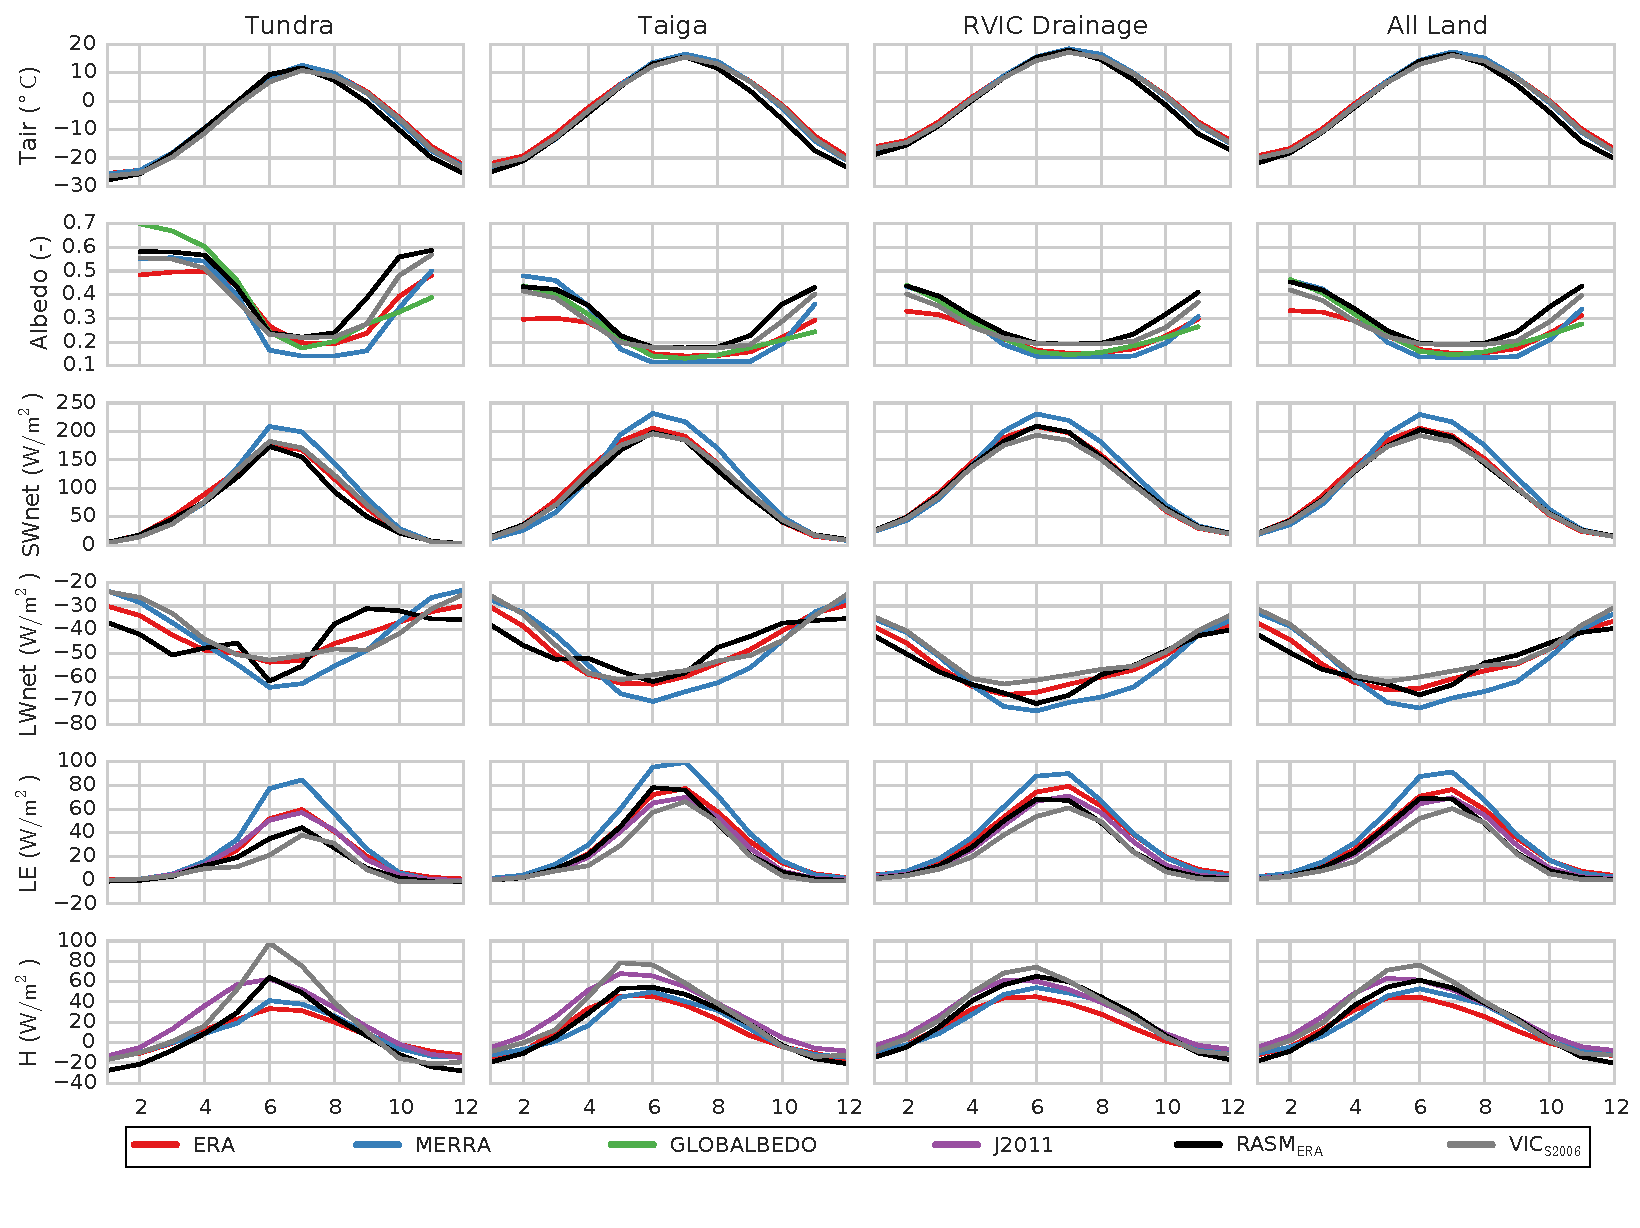
\includegraphics[width=12cm,keepaspectratio]{ch3_Fig3}
  \caption{Average annual cycles of surface air temperature (Tair), albedo, net shortwave radiation (SWnet), net longwave radiation (LWnet), latent heat (LE), and sensible heat (H) for tundra, taiga, the RVIC drainage, and the full model domain for the time period of September 1989–August 2014.}
  \label{fig:energy_cycle}
\end{figure}

\subsection{Radiative fluxes}

The annual cycle of downward shortwave radiation has a large amplitude at high latitudes, with some polar regions receiving less than 30 W m$^{−2}$ in the winter and more than 300 W m$^{−2}$ in the summer.
While clear-sky downward shortwave radiation is only a function of season and latitude, the downward shortwave radiation at the surface also depends on cloud amount and details of the cloud microphysics, which depend on interactions between the atmospheric model boundary layer, microphysics, and radiative transfer schemes.
In RASM, midlatitudes receive 30–50 W m$^{−2}$ more downward shortwave than in ERA, MERRA, and $S2006$, while higher latitudes generally receive less, especially in summer (Fig. S1 in the supplemental material).
In general, the biases in downward radiation in RASM result from too few clouds over midlatitude land areas throughout the year.
The nature of these biases is discussed in detail by \citet{Cassano_2016}.

Reflected shortwave radiation is controlled by the surface albedo, which in the Arctic is mainly determined by the presence or absence of snow.
In the spring, when much of the region is still snow covered, downward shortwave radiation increases rapidly.
Much of this radiation is reflected due to the high albedo of the snow-covered land surface.
RASM captures the difference in cold season albedos between the taiga and tundra, with typical values of 0.4 and 0.6 respectively (Fig. \ref{fig:energy_cycle}).
Compared to the GlobAlbedo product, model simulated surface albedos from RASM, $VIC_{S2006}$, and ERA each have cold season differences that can be as large as +0.25.
Furthermore, all models tend to simulate an early and exaggerated increase in autumn albedo.

Downward longwave radiation is a function of cloud amount, cloud microphysics, and atmospheric temperature and humidity.
Downward longwave radiation is largest in the summer and at midlatitudes (Fig. S3 in the supplemental material).
In the fall and winter seasons at high latitudes, RASM has less downward longwave radiation than ERA, MERRA, and $S2006$, which is driven in part by the cold biases shown in Fig. \ref{fig:temp_maps}, but also contributes to these differences \citep{Cassano_2016}.
The negative downward longwave radiation biases at lower latitudes are mainly due to RASM simulating too few clouds over land areas despite the warm air temperature bias in this region in summer.
Upward longwave radiation is solely a function of the radiative temperature of the land surface, and follows a spatial pattern that is similar to the surface air temperature (Fig. S4 in the supplemental material).
The negative bias in upward longwave in Siberia is reflective of the cold bias in this area.

The combination of downward shortwave and downward longwave radiation is referred to as the total downward radiation and shown in Fig. \ref{fig:drad_maps}.
Total downward radiation has a large seasonal amplitude and a strong zonal gradient, with winter minima at high latitudes less than 150 W m$^{−2}$, and summer maxima at midlatitudes more than 700 W m$^{−2}$.
Compared to ERA and $S2006$, RASM has positive biases at midlatitudes and negative biases at high latitudes, a combination of the previously discussed biases in downward shortwave and longwave radiation.

\begin{figure}
  \centering
  \includegraphics[width=12cm,keepaspectratio]{ch3_Fig4}
  \caption{Seasonal and annual total downward radiation statistics for September 1989–August 2014.
  (top) $RASM_{ERA}$ averages (bottom-left color bar); (second row) $RASM_{ERA}$ std dev (bottom-center color bar); and (next three rows, from top to bottom) $RASM_{ERA}$ biases compared to $S2006$, ERA, and MERRA (bottom-right color bar).}
  \label{fig:drad_maps}
\end{figure}

Net radiation is the difference between total downward radiation and the sum of upward longwave radiation and reflected shortwave radiation.
At high latitudes, average annual net radiation is negative (from −30 to −50 W m$^{−2}$) across most of the pan-Arctic region in the winter (Fig. \ref{fig:nrad_maps}).
Over most of the domain, the net radiation at the surface in RASM is within 15 W m$^{−2}$ of $VIC_{S2006}$, MERRA, and ERA.

\begin{figure}
  \centering
  \includegraphics[width=12cm,keepaspectratio]{ch3_Fig5}
  \caption{Seasonal and annual net radiation statistics for September 1989–August 2014.
  (top) $RASM_{ERA}$ averages (bottom-left color bar); (second row) $RASM_{ERA}$ std dev (bottom-center color bar); and (next three rows, from top to bottom) $RASM_{ERA}$ biases compared to $VIC_{S2006}$, ERA, and MERRA (bottom-right color bar).}
  \label{fig:nrad_maps}
\end{figure}

\subsection{Turbulent fluxes}

Surface turbulent heat fluxes are perhaps the least constrained flux variables in coupled land–atmosphere models.
Estimates of sensible and latent heat flux from the MERRA and ERA reanalysis products are computed entirely within the reanalysis land surface model and are not directly constrained by data assimilation.
\citet{Lindsay_2014} highlight that point in their intercomparison of seven reanalysis products over the pan-Arctic domain, citing intermodel variations in the seasonal sensible and latent heat fluxes in some regions on the order of 50 W m$^{−2}$.
RASM and the reanalysis products simulate a regional maximum latent heat flux across the taiga in the summer (Fig. \ref{fig:energy_cycle}).
In RASM, the sensible heat flux in the midlatitudes is from +10 to +40 W m$^{−2}$ greater than in ERA and MERRA during summer.
RASM latent heat fluxes tend to be lower than both ERA and MERRA but are closer to the empirical estimates of J2011 (Fig. S5 in the supplemental material).

The annual cycle of the latent heat flux is largely driven by the seasonal cycle of net shortwave radiation.
In the winter season (DJF), the latent heat flux is nearly zero across the entire RASM domain (Fig. S5).
The latent heat flux is largest in the summer over the taiga, with a seasonal averaged latent heat flux near 80 W m$^{−2}$.
The spatial distribution of the seasonally averaged latent heat flux varies substantially among models (e.g., RASM, MERRA, and ERA).
Local differences in the simulated latent heat flux can be as large as 50 W m$^{−2}$.
Averaged over the taiga, the summer season (JJA) latent heat flux is more than +20 W m$^{−2}$ larger in MERRA than in the RASM, ERA, or J2011 datasets.
As discussed below, these differences in the latent heat flux are consistent with the differences in the partitioning of evapotranspiration and runoff.

The sensible heat has a more distinct zonal gradient than the latent heat flux, with the largest sensible heat fluxes in the southern portions of the domain (Fig. S6 in the supplemental material).
This gradient is stronger in RASM than in MERRA, ERA, or J2011.
The differences in the sensible heat flux when compared to MERRA and ERA are closely related to the differences in total downward radiation.
RASM simulated winter season sensible heat is negative over most of the domain, especially over the high latitudes.
A negative sensible heat flux represents an energy flux from the atmosphere to the land surface or heating of the land by the atmosphere.
The ERA, MERRA, and J2011 datasets agree with this behavior although the spread among the models is as large as 30 W m$^{−2}$.
Intermodel differences in the sensible heat flux can be as large as the differences in the latent heat flux.
In the case of RASM, the biases have a zonal structure that is likely tied to biases in downward radiation rather than vegetation.

In the tundra and taiga regions, the sensible heat flux characteristically peaks about a month earlier than the latent heat flux.
This process is primarily due to large amounts of downward radiation over a mostly snow-covered land surface, which inhibits evapotranspiration \citep{Betts_2001}.
Figure \ref{fig:energy_cycle} demonstrates that RASM follows this asymmetry in the turbulent fluxes.

\subsection{Hydrologic fluxes}

Figure \ref{fig:prec_maps} shows the spatial distribution of RASM precipitation.
The spatial pattern of precipitation in the Arctic is highly heterogeneous.
Significant portions of the domain receive less than 300 mm yr−1 (0.8 mm day$^{−1}$), while some coastal and midlatitude regions receive over 1500 mm yr−1 (4.1 mm day$^{−1}$).
Precipitation is largest in the summer across most of the pan-Arctic region.
In most cases, RASM simulates larger amounts of orographic precipitation (e.g., west coast of North America) compared to MERRA and ERA, likely as a result of its higher spatial resolution and therefore greater ability to resolve topography.


\begin{figure}
  \centering
  \includegraphics[width=12cm,keepaspectratio]{ch3_Fig6}
  \caption{Seasonal and annual precipitation statistics for September 1989–August 2014.
  (top) $RASM_{ERA}$ averages (bottom-left color bar); (second row) $RASM_{ERA}$ std dev (bottom-center color bar); and (next four rows, from top to bottom) $RASM_{ERA}$ biases compared to $S2006$, ERA, MERRA, and A2006 (bottom-right color bar).}
  \label{fig:prec_maps}
\end{figure}

We compared the basin average precipitation for four basins (Fig. \ref{fig:domain}c) with four reanalysis and observation based datasets (Fig. \ref{fig:water_cycle}).
RASM effectively captures the seasonal cycle of precipitation, with the largest precipitation amounts in the summer season.
While most of the datasets show similar amounts of accumulated cold-season precipitation, $S2006$ stands out as being particularly dry, leading to less snow accumulation.
The annual cycle of runoff in the Arctic is driven by spring snowmelt and summer precipitation.
RASM captures this pulse in melt season runoff in each of the basins shown in Fig. \ref{fig:water_cycle}.
For $RASM_{ERA}$, $VIC_{S2006}$, ERA, and MERRA there are significant differences in seasonality of basin-averaged runoff compared to R-ArcticNET with the spring freshet in most datasets preceding the observations by 1–2 months.

\begin{figure}
  \centering
  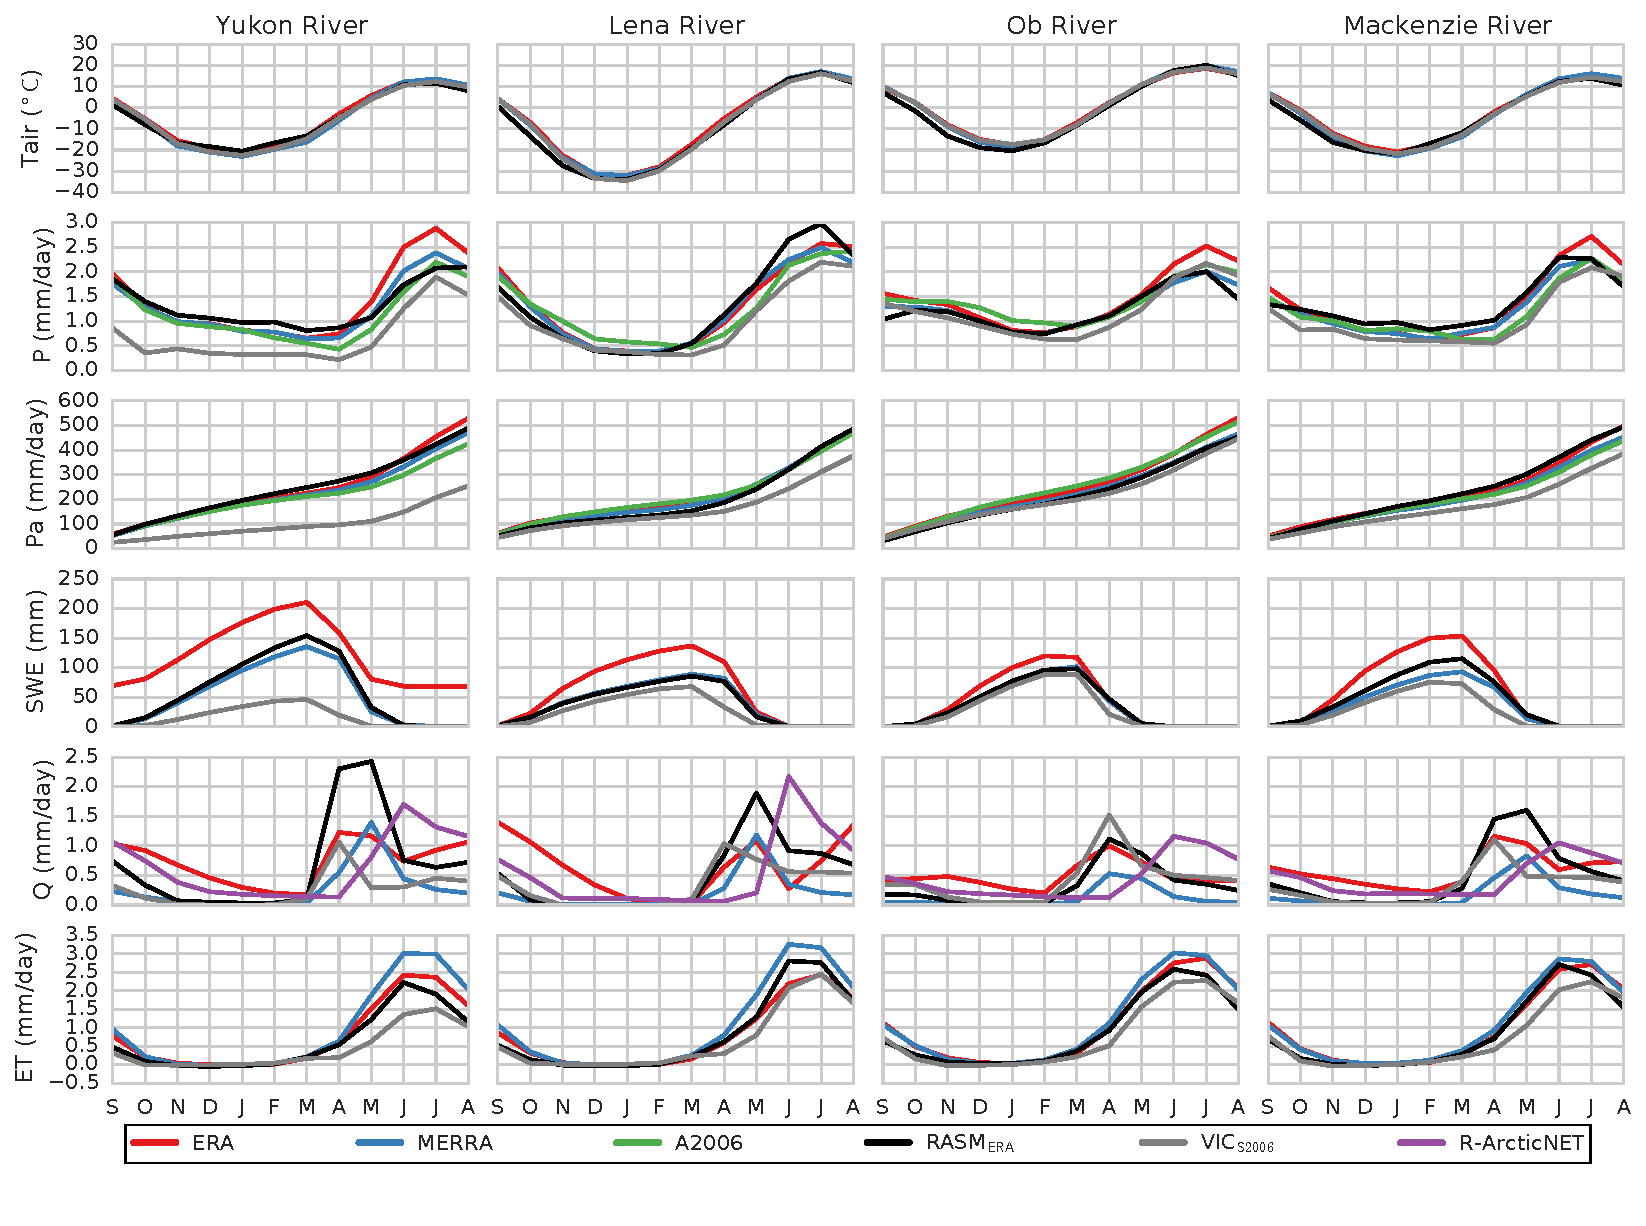
\includegraphics[width=12cm,keepaspectratio]{ch3_Fig7}
  \caption{Average annual cycles of Tair, precipitation (P), accumulated precipitation (Pa), snow water equivalent (SWE), streamflow (Q), and evapotranspiration (ET) for four of the largest river basins in the RASM domain for the time period of September 1989–August 2014.}
  \label{fig:water_cycle}
\end{figure}

\subsection{Snow}

Winter and spring snow cover influence the regional and global climate through increased surface albedo, the latent heat required for melting and sublimation, and the freshwater flux into the Arctic during late spring and summer.
Basin-averaged snow water equivalent (SWE) in RASM shows seasonal accumulation and ablation patterns that are similar to MERRA and ERA.
Basin-averaged differences correspond largely to differences in cool season precipitation (Fig. \ref{fig:water_cycle}).
The annual cycle of basin-averaged snow water equivalent in RASM is generally closer to that of MERRA than ERA.

Figure \ref{fig:snow} compares snow cover north of 50$^{\circ}$N (defined in RASM and the reanalysis products as grid cells with average SWE >1 mm) to the National Snow and Ice Data Center weekly snow cover data product.
Note that the uncertainty in the satellite estimated snow cover extent is on the order of 5\%–10\% in the spring \citep{Brown_2011}.
Additional uncertainty is introduced in our analysis through the comparison between model snow cover derived using a grid cell average SWE threshold and remote sensing estimates of snow cover.
RASM simulated snow cover extent north of 50$^{\circ}$N reaches a maximum by the start of January and a minimum by the end of June.
RASM’s increase in snow-covered area in fall closely follows the MERRA and NSIDC datasets and its onset of spring melt matches NSIDC.
However, RASM simulations show a shorter ablation period, especially at high latitudes in North America and eastern Siberia between May and June, where the retreat of snow-covered area in RASM precedes satellite observations by about 15 days.
Accompanying this more rapid retreat of high-latitude snow cover is a warm bias in May and June in those regions.
Increase in snow-covered area in the $VIC_{S2006}$ simulation lags by more than 10 days, whereas the decrease precedes that of the other dataset due to less precipitation in $S2006$ compared to the other datasets (see also Figs.
\ref{fig:water_cycle} and \ref{fig:snow}).


\begin{figure}
  \centering
  \includegraphics[width=12cm,keepaspectratio]{ch3_Fig8}
  \caption{Number of snow-covered days per year for (top left) RASM and (top right) NSIDC.
  (bottom left) Difference between numbers of snow-covered days per year in (top).
  (bottom right) Annual cycle of snow-covered area north of 50$^{\circ}$N.
  Time period is September 1989–August 2014.}
  \label{fig:snow}
\end{figure}

\section{Discussion}
\label{sec:discussion_ch3}

In uncoupled land surface simulations, models are frequently evaluated on the basis of their ability to capture key terms in the hydrologic cycle, such as snow water equivalent, streamflow, soil moisture, and evapotranspiration.
These models are often calibrated using objective functions that target only one or two of these variables.
In many cases, these calibrations, or parameter selection techniques, achieve good statistical representation of the target variables without additional assessment of the remaining fluxes and states in the model.
In the process of developing the VIC–WRF coupling in RASM, we have found it necessary to take a holistic approach to assess model performance.
Our focus has been on improving the representation of individual processes and understanding how individual processes contribute to the climate system rather than achieving an optimal calibration.

The land surface is coupled to the atmosphere via three primary mechanisms: surface radiation exchange, turbulent heat flux exchange, and the partitioning of precipitation into evapotranspiration and runoff.
Our analysis of the surface energy budget in the RASM domain indicates that differences in the downward radiation forcings (±50 W m$^{−2}$), compared to reanalysis and $S2006$, may be large enough to affect the land surface model performance.
An example of this is in western Siberia during the winter and fall when RASM shows less downward longwave radiation than the reanalysis products, leading to local surface air temperature biases between −4$^{\circ}$ and −8$^{\circ}$C as compared to ERA.

The largest control on the terrestrial surface energy budget is the surface albedo.
During winter and spring, the tundra is snow-covered and its albedo can be 6 times higher than in the adjacent taiga \citep{Chapin_2000b} where vegetation with much lower albedo protrudes through the snow.
Early RASM simulations did not include a vegetation-dependent maximum snow albedo, resulting in cool season albedos in vegetated areas that were much higher than observations.
These high values in surface albedo were accompanied by negative surface air temperature biases over much of the tundra and taiga that were as large as −10$^{\circ}$C.
Applying a vegetation-dependent maximum snow albedo resulted in a lower surface albedo (Fig. \ref{fig:albedo_maps}) and reduced the surface air temperature bias throughout the cool season.
These results extend the findings of \citet{Viterbo_1999}, who reduced the snow-covered vegetation albedo from 0.8 over the taiga to 0.2 in ECMWF’s global forecast model resulting in a reduction of surface air temperature bias from more than −8$^{\circ}$C to less than −2$^{\circ}$C.

\begin{figure}
  \centering
  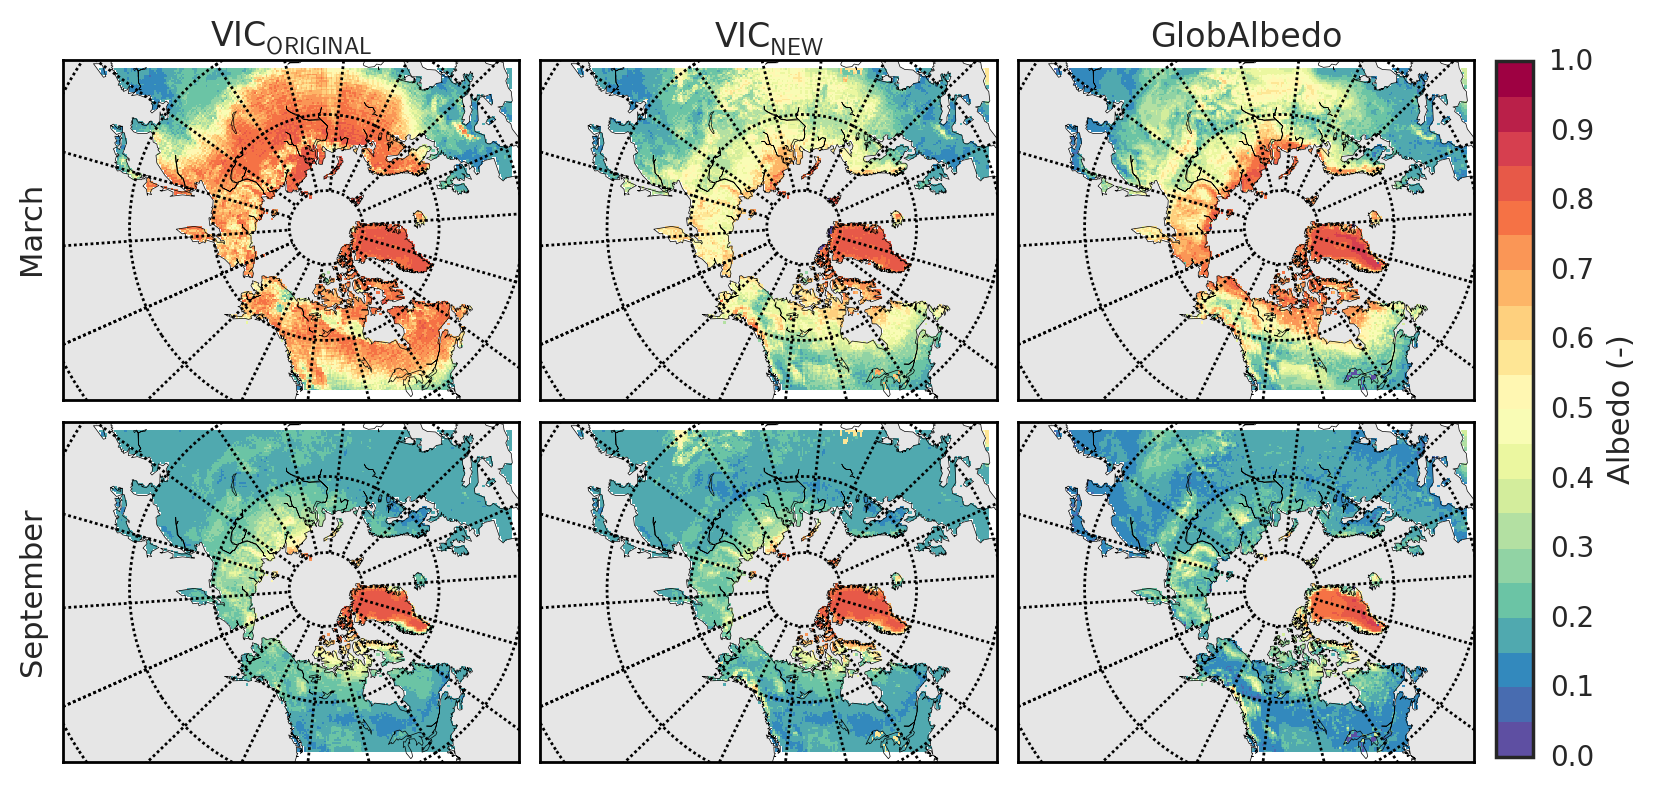
\includegraphics[width=12cm,keepaspectratio]{ch3_Fig9}
  \caption{Surface albedos for (top) March and (bottom) September for (left) the original VIC albedo schemes, (center) the albedo schemes used in RASM (e.g., VICNEW), and (right) the GlobAlbedo remote sensing product.
  Time period is 1998–2007.}
  \label{fig:albedo_maps}
\end{figure}

Observational studies, such as \citet{Beringer_2005}, have shown that the tundra and taiga biomes partition the warm season turbulent heat fluxes differently.
Across the taiga regions, we expect Bowen ratios to be much greater than one in the spring and near one in the summer (Fig. \ref{fig:bowen}).
In the tundra regions, we expect growing season (JJA) Bowen ratios of less than one.
In the taiga, RASM captures the spring peak in the Bowen ratio with an average value of 1.13 and the decline in summer with an average value of 0.76 (see Table S5 in the supplemental material).
In the tundra during the summer, RASM tends to have a higher than expected Bowen ratio of 1.55.
During the fall, turbulent fluxes tend to be small and RASM, ERA, and MERRA register negative Bowen ratios, resulting from a negative sensible heat flux.
Comparing RASM, ERA, and MERRA to the spatial patterns found in the empirical estimates of J2011, we find that ERA and MERRA tend to have much lower Bowen ratios across much of the domain during all three seasons.
This is particularly apparent during the spring and summer months in the high latitude tundra portions of the domain, where RASM and J2011 both show Bowen ratios near or above 1.0 while ERA and MERRA are consistently below 1.0.

\begin{figure}
  \centering
  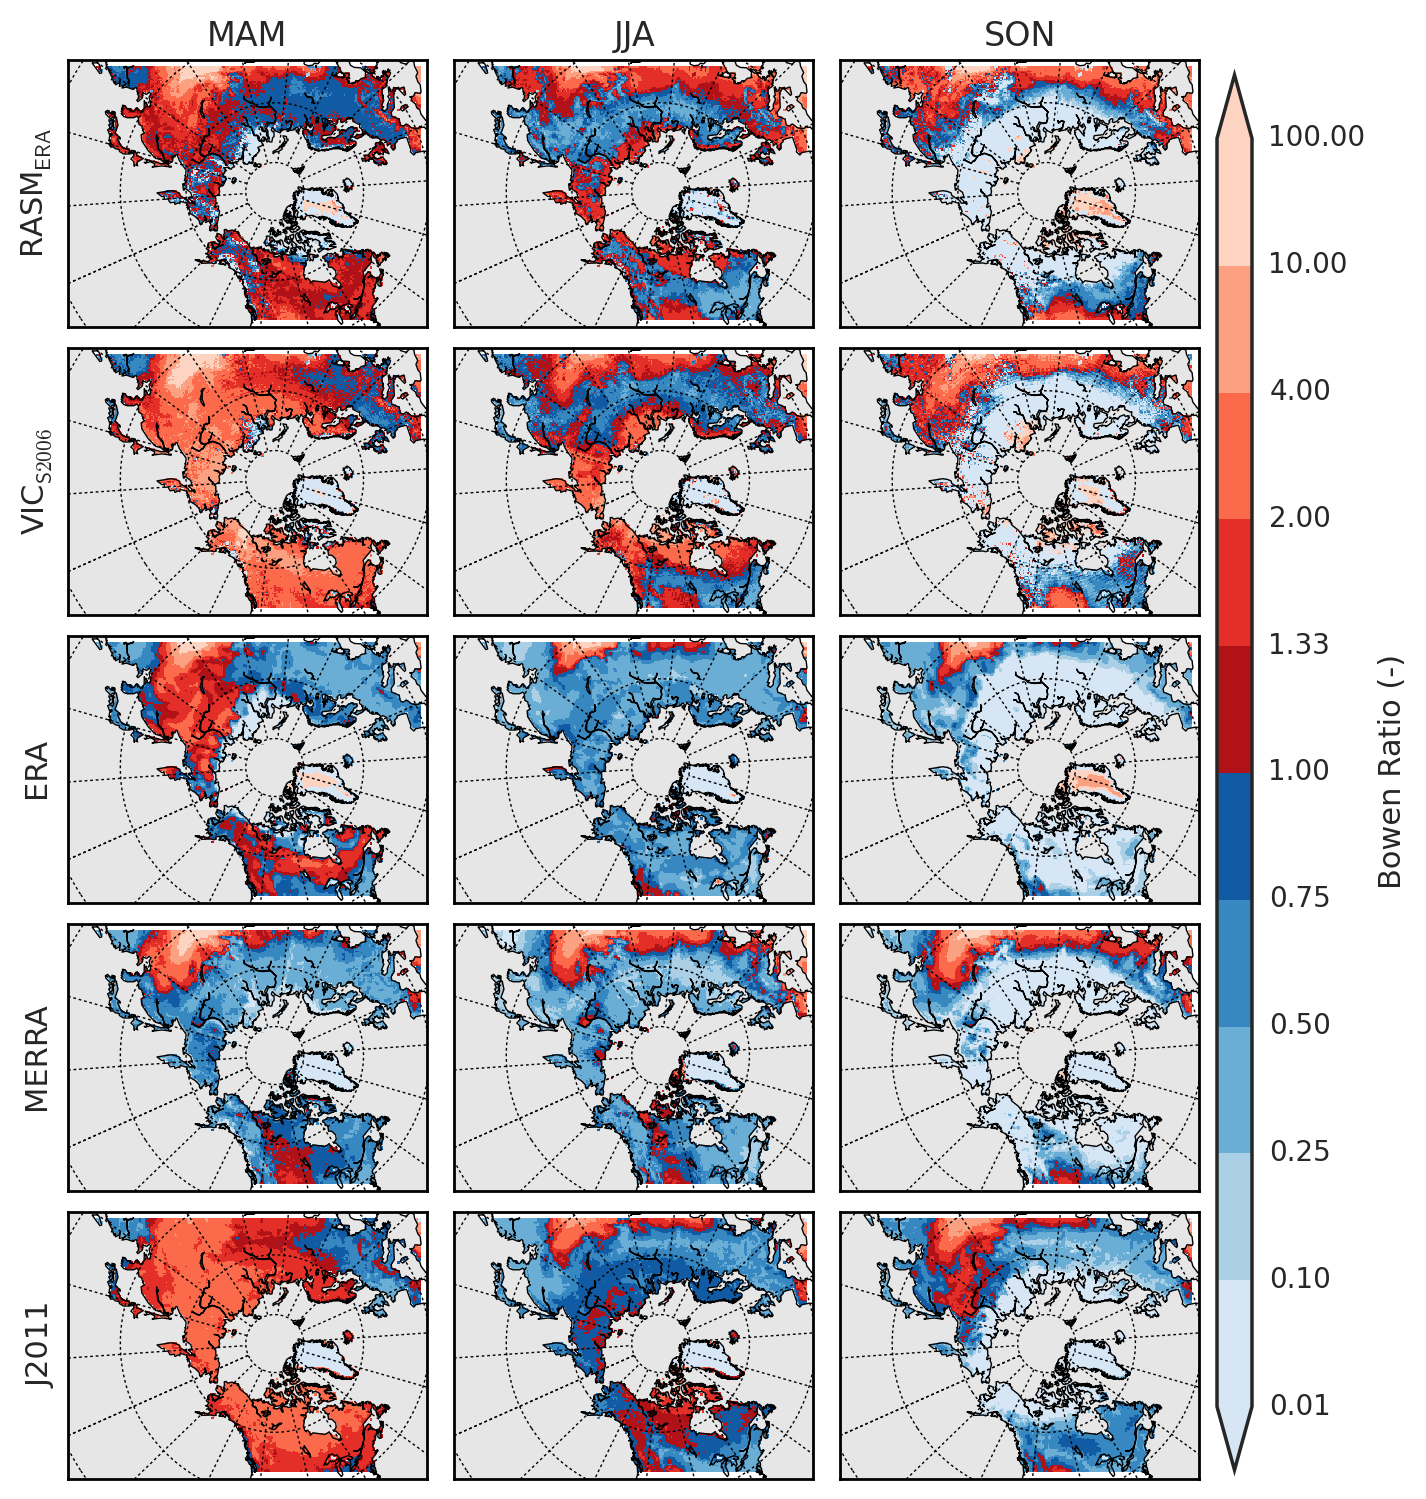
\includegraphics[width=15cm,keepaspectratio]{ch3_Fig10}
  \caption{Spring, summer, and fall Bowen ratios for $RASM_{ERA}$, $VIC_{S2006}$, ERA, MERRA, and J2011 for the time period of September 1989–August 2014.}
  \label{fig:bowen}
\end{figure}

The turbulent heat fluxes, along with heat storage, balance net radiation at the surface.
The partitioning of the turbulent heat fluxes between latent heat and sensible heat is a function of the stability of the boundary layer and the availability of mobile liquid water at or below the surface.
In the pan-Arctic region, the seasonal and diurnal cycles of the sensible and latent heat fluxes vary considerably by land cover types.
To highlight RASM’s ability to simulate the turbulent heat fluxes, we compared the diurnal cycles at two flux tower locations to the nearest RASM grid cells.
This analysis serves to demonstrate that RASM simulates the diurnal cycle with close resemblance to point observations, particularly with respect to the magnitude and timing of the diurnal cycle and the relative importance of the individual fluxes.
Figure \ref{fig:diurnal_cycle} shows the observed July-averaged (1994 and 1995) diurnal cycle at the Boreal Ecosystem Atmosphere Study \citep[BOREAS; ][]{Sellers_1997} Old Black Spruce \citep{Barr_2006} and the Happy Valley, Alaska \citep{Eugster_2000}, flux tower locations (Fig. \ref{fig:domain}d) compared to the RASM-simulated diurnal cycle at the nearest grid cell location.
The BOREAS and Happy Valley sites are representative of the taiga and tundra locations, respectively.
RASM’s diurnal temperature range (DTR) at the BOREAS site is similar to the observed DTR (about 10$^{\circ}$C) despite being about 2$^{\circ}$C colder on average.
At the tundra site, however, the RASM-simulated DTR (about 5$^{\circ}$C) is much smaller than the observed 9$^{\circ}$C.
At both locations, net radiation is similar to the observations in terms of magnitude and diurnal timing and is mostly determined by the atmospheric forcing of downward radiation.
The timing of the diurnal cycle of the latent heat and the sensible heat fluxes in RASM is similar at both the taiga and tundra sites, and the differences in the magnitude are typically less than 40 W m$^{−2}$.
Averaged over the month of July, RASM and observed Bowen ratios at the BOREAS site were 0.89 and 1.27, respectively, and were 0.88 and 0.69 at the Happy Valley site.

\begin{figure}
  \centering
  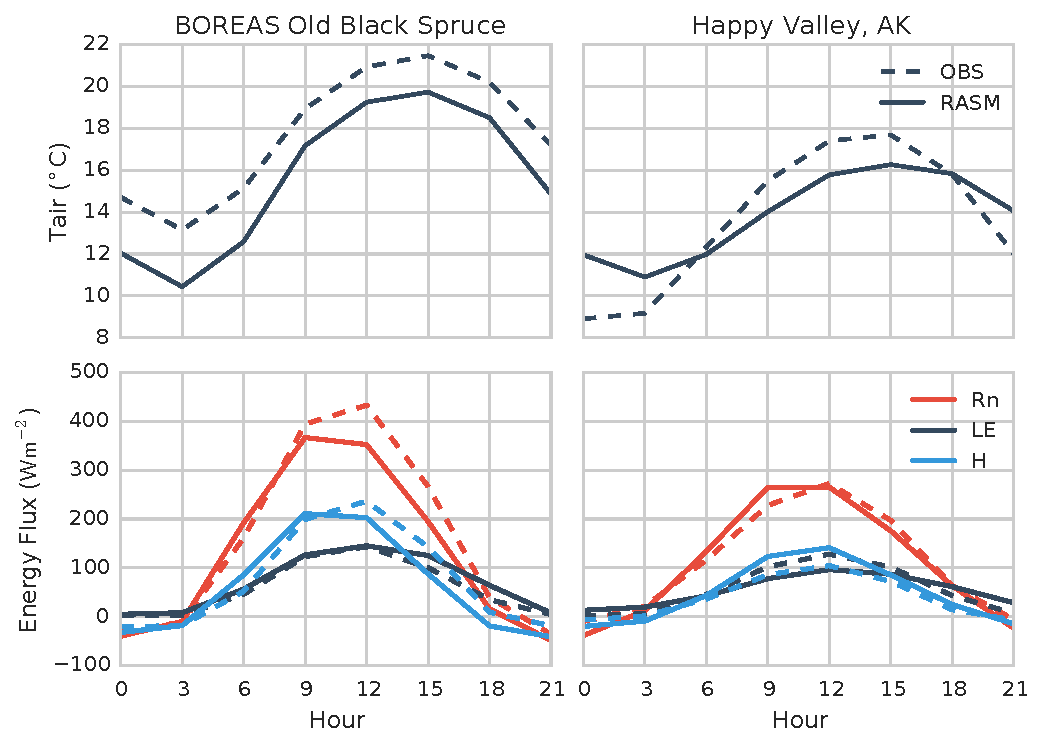
\includegraphics[width=10cm,keepaspectratio]{ch3_Fig11}
  \caption{(top) Averaged diurnal cycle of Tair and (bottom) net radiation (Rn), LE, and H for July at the (left) BOREAS Old Black Spruce and (right) Happy Valley, Alaska, flux tower locations based on observations (OBS; dashed line) and RASM (solid line).
  RASM results are based on the simulated values at the nearest grid cell location.
  Time period is July 1994 and 1995.}
  \label{fig:diurnal_cycle}
\end{figure}

On annual time scales, surface and subsurface runoff from the land surface can be thought of as the difference between precipitation and evapotranspiration, assuming no change in storage.
Since we lack the ability to effectively measure evapotranspiration across large areas, in situ observations of streamflow and gridded observations of precipitation enable us to evaluate the overall water balance.
Figure \ref{fig:streamflow_scatter} shows climatological, basin-averaged precipitation, runoff, and runoff ratios from the A2006 precipitation and R-ArcticNET (Fig. \ref{fig:domain}d) runoff datasets and compares these to the same quantities based on $RASM_{ERA}$, $VIC_{S2006}$, MERRA, and ERA.
Compared to A2006 precipitation, $RASM_{ERA}$ has the lowest root-mean-square error (RMSE) and bias of all the models, +0.3 and +0.0072 mm day$^{−1}$ respectively.
$VIC_{S2006}$, which is forced using $S2006$, has a negative bias (−0.34 mm day$^{−1}$) compared to A2006, especially in wetter basins (those with precipitation greater than 1.75 mm day$^{−1}$).
All of the datasets are biased low with respect to runoff compared to R-ArcticNET.
$RASM_{ERA}$ and ERA have the smallest biases, −0.12 and −0.021 mm day$^{−1}$, respectively, while the $VIC_{S2006}$ and MERRA datasets have biases of −0.3 and −0.4 mm day$^{−1}$, respectively.
Although the differences in precipitation between MERRA and A2006 are not large, annual runoff from MERRA is substantially lower than observed at nearly all gauge locations, indicating systemic overestimation of evapotranspiration (and thus the latent heat flux) in MERRA.
This finding aligns with the results shown in Figs. \ref{fig:snow} and \ref{fig:bowen}, in which MERRA is shown to have larger evapotranspiration and latent heat fluxes and smaller Bowen ratios than RASM or ERA.
\citet{Shiklomanov_2006} estimated annual runoff measurement errors in the largest six Eurasian rivers between 1.5\% and 3.5\%.
If we apply these error estimates across the entire R-ArcticNET dataset, we find that measurement errors are about an order of magnitude smaller than the biases shown in Fig. \ref{fig:streamflow_scatter}.
Compared with the combination of A2006 and R-ArcticNET runoff, all models have considerably more scatter in their runoff ratio than they do for runoff or precipitation alone (Fig. \ref{fig:streamflow_scatter}).
RASM, ERA, and $VIC_{S2006}$ overpredict low runoff ratios and underpredict high runoff ratios while MERRA is consistently biased low.


\begin{figure}
  \centering
  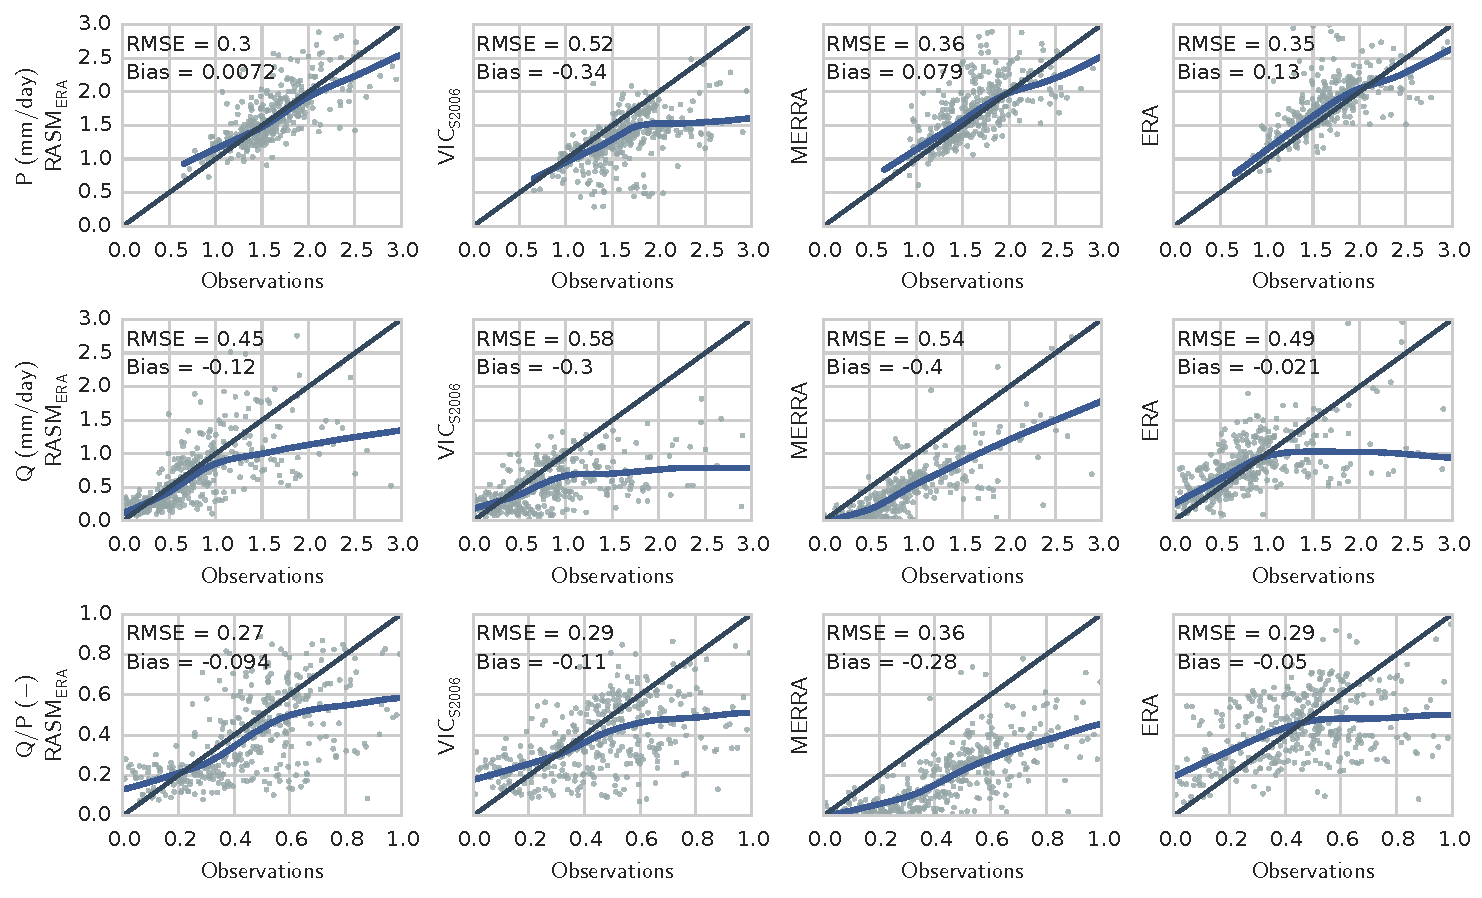
\includegraphics[width=10cm,keepaspectratio]{ch3_Fig12}
  \caption{Comparison of observed P from A2006 and Q from R-ArcticNET to $RASM_{ERA}$, $RASM_{CFSR}$, $VIC_{S2006}$, MERRA, and ERA at 379 individual basins.
  The blue line is a locally weighted scatterplot smoothing (LOWESS) best-fit model.
  The RMSE (mm day$^{−1}$) and bias (mm day$^{−1}$) statistics are shown in the top-left corner of each panel.
  Climatological mean of coincident records between September 1980 and August 2014.}
  \label{fig:streamflow_scatter}
\end{figure}

The energy and water cycles are linked through the latent heat flux.
The partitioning of precipitation into runoff and evapotranspiration is also directly related to the latent heat flux.
We have shown large intermodel differences in the runoff ratio, especially between RASM and MERRA.
RASM and ERA tend to have similar runoff generation behavior on annual time scales and also tend to match the global J2011 dataset well.
Conversely, MERRA tends to have very low runoff ratios and considerably higher latent heat fluxes in the spring and summer compared to J2011.
ERA’s annually averaged runoff tends to match observations reasonably well, despite having slightly greater precipitation in the spring and summer \citep[see Fig. \ref{fig:streamflow_scatter} herein; ][]{Lindsay_2014}.
While considering the evapotranspiration flux from MERRA and ERA, it is worth remembering that both models assimilate observations of humidity in the troposphere and thus, by design, eliminate most of the feedback mechanisms between evapotranspiration and precipitation.
This explains in part why MERRA’s precipitation is reasonable despite more evapotranspiration than ERA or RASM.

The need to evaluate land surface model performance in a coupled environment is demonstrated by the substantial differences in model results between the coupled and uncoupled VIC simulations ($RASM_{ERA}$ and $VIC_{S2006}$), distinctions that warrant further investigation.
For example, in the coupled environment, biases in atmospheric forcings, such as the cold season negative bias in downward longwave radiation in $RASM_{ERA}$, result in biases at the land surface and feedbacks to the atmosphere through the surface energy budget.
In the uncoupled environment, the atmospheric forcing is prescribed so that most of the land–atmosphere feedback processes are ignored.

\section{Conclusions}
\label{sec:conclusions_ch3}

The development of RASM has been motivated by the need to improve multidecadal climate simulations in the pan-Arctic region and to improve understanding of the coupled climate system.
We coupled the VIC land surface model within the CESM infrastructure and compared land surface fluxes and states to uncoupled simulations, reanalysis datasets and observation-based products to provide a baseline evaluation of the land surface climate in RASM version 1.0.
Based on these comparisons, we have shown that RASM reproduces many important aspects of the Arctic land surface climate, such as the amount and regional distribution of precipitation and its partitioning between runoff and evapotranspiration, the effects of snow on the water and energy balance, and the differences between the main tundra and taiga biomes in simulated turbulent fluxes.
We also compared RASM to the reanalyses ERA and MERRA.
In comparisons with assimilated variables, such as surface air temperature, we found that RASM reproduces the spatial patterns and seasonal cycle well, although there are large local differences and RASM has a larger seasonal amplitude overall.
With respect to derived variables, such as latent heat or runoff, we found that RASM, in comparison to observation-based datasets, performs as well as or better than ERA or MERRA.
We have also shown that there are specific aspects in the land surface component that can be improved.
For example, while the annual cycle of snow-covered area in RASM compares well to satellite observations, the melt progresses faster in the late spring at high latitudes.

The partitioning of the hydrologic fluxes varies among $RASM_{ERA}$, ERA, and MERRA.
For example, $RASM_{ERA}$ and ERA tend to agree on the annual runoff ratio, but demonstrate substantially different seasonal runoff behavior, with RASM simulating a well-defined runoff peak in April or May and ERA simulating a smaller spring runoff peak with more runoff throughout the summer and autumn.
Conversely, MERRA has very low runoff ratios and the largest amount of evapotranspiration.
We have found that these relationships can also be applied to the surface energy budget.
Among $RASM_{ERA}$, ERA, and MERRA, we have found a wide range in the sensible and latent heat fluxes.
MERRA tends to have a larger latent heat flux and a smaller Bowen ratio than $RASM_{ERA}$ and ERA, which is consistent with MERRA’s low runoff ratio.

Ongoing development of the RASM land surface and land–atmosphere coupling includes improved treatment of ground heat flux and canopy processes, increased spatial resolution, and coupling of new submodel components including a subgrid glacier model and a dynamic vegetation model.

{\bf Acknowledgments}
This research was supported under U.S. Department of Energy (DOE) Grants DE-FG02-07ER64460 and DE-SC0006856 to the University of Washington, and DE-SC0006178 to the University of Colorado.
Supercomputing resources were provided through the Department of Defense (DOD) High Performance Computing Modernization Program at the Army Engineer Research and Development Center and the Air Force Research Laboratory.
We would also like to thank José Renteria and Kevin Lind for their early contributions to the coupling of VIC within RASM, work that was funded through the DOD user Productivity, Enhancement, Technology Transfer, and Training (PETTT) program.
